\chapter{Methods\label{methods}}
This chapter aims to establish a precisely defined and rigorous research approach to enhance transparency and repeatability. We will take the steps required to ensure that every phase and decision is thoroughly documented, enabling the reader to retrace the research process. In a thesis made by a single researcher, the lack of cross-examination of results with multiple researchers and the validation of evaluation criteria for opinion bias pose threats to validity, as will be clarified further in \hyperref[discussion]{Chapter 4}. Therefore, special attention will be paid to address these concerns. By following this approach, this research endeavors to contribute to the existing body of knowledge in the field of computer science in a robust and reliable manner.

The systematic literature review method is a well-established approach for conducting a comprehensive and rigorous analysis of the existing research on specific research question or subject \citep{kitchenham2007}. This paper presents a multivocal literature review. Multivocal literature review is type of systematic literature review that includes both academic literature and grey literature \citep{mantyla2019}. This method was selected for this study to facilitate a thorough and scientifically interdisciplinary examination of public licenses in software engineering. The existing literature consists of public software licenses not found in academic databases and as such are considered gray literature, making the thesis a multivocal literature review.

This study follows the guidelines outlined by \cite{kitchenham2007}, to ensure its quality. The multivocal review method consists of three distinct phases: planning, conducting and reporting the review. This study stricly adhered to this structure. The phases can be further broken down into a research protocol, as illustrated in \hyperref[fig:slrphases]{Figure 2.1}. Adhering to the protocol is the first step in ensuring a well-documented and rigorous process, which increases the validity and auditability of the study.

\begin{figure}
	\centering
	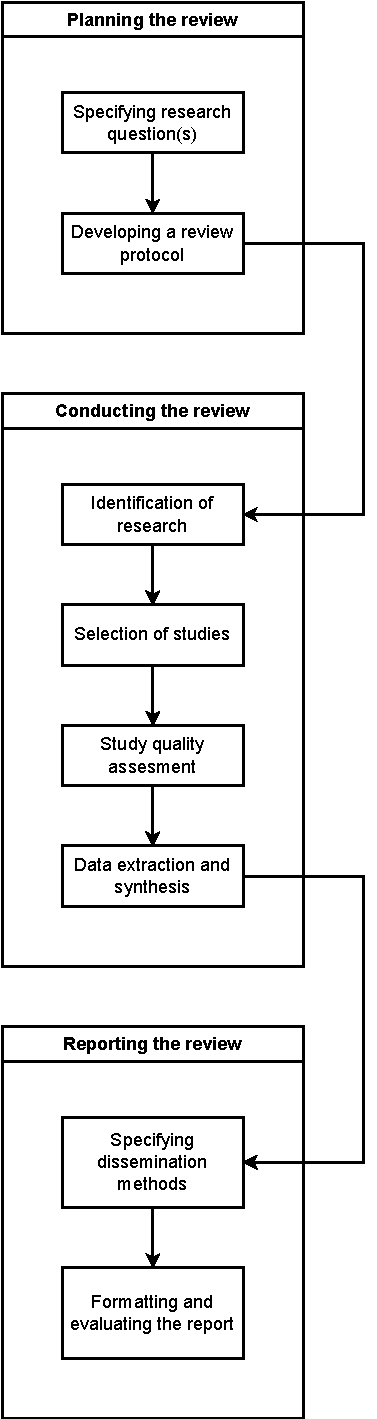
\includegraphics[scale=0.9]{figures/slr-phases.pdf}
	\caption{Three phases of a systematic literature review}
	\label{fig:slrphases}
\end{figure}

The multivocal literature review process began with the formulation of research questions and the establishment of a comprehensive search strategy and scope. The search process was conducted by employing a quasi-gold standard (QGS) approach based on the implementation by \cite{qgs}. After the completion of the search process, the inclusion and exclusion criteria were defined. To ensure a structured evaluation of the literature, a data extraction form was created. Finally, a strategy for analyzing the extracted data from the literature was designed.

 To ensure the reliability and validity of the research protocol, it was validated against similar systematic literature reviews in computer science, the aforementioned guidelines by \cite{kitchenham2007}, and was further refined through an iterative process. Specifically, a subset of the data was tested on (The QGS) and any identified issues or problems were recorded and addressed. The details of this process are explained and thoroughly documented in the following sections. Similarly, the same approach was followed for the data extraction process, whereby a subset of literature was tested to refine the data extraction form. The revision of the form was undertaken as necessary to guarantee the completeness and accuracy of the extracted data.

\section{Research questions}
The research questions in this study served two primary purposes. Firstly, they aimed to provide an analysis of the existing multivocal literature on public licenses in software engineering for the researchers interested about the field. Secondly, the questions were designed to cater a secondary audience of professional software engineering practicioners. As discussed in the \hyperref[intro]{Chapter 1}, the following research questions were addressed in this thesis:

\begin{itemize}
  \item RQ1: How many public licenses in software engineering does there exist?
  \item RQ2: How consistent are the naming conventions for public licenses in software engineering
  \item 
\end{itemize}

The multivocal literature review in this thesis begins with addressing RQ1, which aims to provide the amount of public software licenses that exist in our five public license listing sites in total. This information could be most valuable to the researchers. The results can be used to introduce some notable background of the current public licenses in software engineering and enabling focus to more specific areas inside the topic of this thesis.

Next RQ2 seeks to find the amount of duplicate licenses between the license listing sites. Results to this research question are also mostly useful to researchers of the field. Moreover, the documented methods are most likely the most valuable information for the researchers.

Finally RQ3 attempts to count the total number of individual public software licenses within the scope of this thesis. The research question builds on top of the results and methods of the previous research questions. This information could be most valuable for the practitioners since it could give some overview and a sense of the scale when picking a public software license that would serve the practitioners' needs the best.

\section{Search strategy}
% where was search process conducted in (inclusion/exclusion in appendix a)
The search process was conducted on five public license listing websites. The selection criteria for the literature were defined after the search process and the selection process was based on inclusion and exclusion criteria. The inclusion and exclusion criteria and each step of exclusion on the literature found are presented later in this chapter. Originally the search terms would have been applied to the license listing sites directly just like in a normal multivocal literature review or in a systematic literature review. Keywords however produced highly varying and non-reproducible results in Google Scholar and Google Search. Some license listing websites such as FSF's list of pages categorized as licenses could not be found from Google Search even with the \texttt{site} operator: \\
\texttt{site:https://directory.fsf.org/wiki/Category:License}. Although the page has been up since 2013, for some reason Google has not crawled the page in 10 years \citep{fsf:licenselist}. This is why this thesis does not include search terms of the initial phase per se but rather inclusion and exclusion strings on the second phase. For the sake of validity the thesis still follows the guidelines presented in \cite{kitchenham2007} with the exception of replacing an academic database search engine with the five license listing sites, web scraping and our own Python script performing the legwork of an academic database search engine in a systematic literature review.

% data extraction process
The data extraction process was performed in a standardized and systematic manner, with the aim of obtaining the relevant information from the selected literature. The data extraction form used included license shortcode used in the listing site, listing site name, full license text and is available  \hyperref[table:extraction]{Table 2.2}. The extracted data was then used to answer the research questions and perform the data analysis. The results of the data analysis were then reported in a rigorous manner.

% more on where was search process conducted in
\subsection{Search method}
The search was conducted on five license listing websites, as mentioned earlier, to obtain a broad set of multivocal literature. This approach yielded a large number of literature that were processed to a subset of high-relevance literature using inclusion and exclusion criteria presented later in this chapter. Manual searching of databases with hundreds of public licenses is not feasible, and it is prone to researcher bias and may overlook relevant venues from other scientific disciplines. However, a preliminary manual search was performed to reduce the number of iterations required and establish the quasi-gold standard (QGS) mentioned earlier.

% how were search terms determined
\subsection{Search scope and terms}
The search terms, or in our case, the inclusion and exclusion string was determined through an iterative process that took into account the research questions and topic. Synonyms for key terms were included and combined using Boolean logic to form a comprehensive inclusion and exclusion string. As mentioned earlier the inclusion and exclusion criteria are presented later in this chapter.

% qgs on search string
The inclusion and exclusion string was established on a basis of quasi-gold standard as proposed by \cite{qgs}. For establishing a quasi-gold standard we employed a manually crafted inclusion and exclusion string based on the topic and research questions of this study. As we defined public licenses in software engineering as licenses where the licensees are not limited and the license in question is meant be used in licensing software source code in \hyperref[intro]{Chapter 1} and our research questions focus on finding useful metrics about the public licenses, we manually formulated the inclusion and exclusion string in Python:
\begin{verbatim}
  ^(?!.*\b(documentation\s+license|creative\s+commons|open data)\b).*
\end{verbatim}
% web scrape beginning
In order to run the inclusion and exclusion string that established the quality-gold standard against the literature we had to gather them first. We started defining our search scope from the Wikipedia page of one of the most used open source license \citep{github:licenseusage}, the MIT license \citep{wikipedia:mit}. The infobox contained fields in the order shown in \hyperref[table:infobox]{Table 2.1}.

\begin{table}[t]
	\begin{center}
		\begin{tabular}{||c c||}
			\hline
			Field & Value \\
			\hline
			Publisher & Massachusetts Insitute of Technology \\
			SPDX identifier & MIT \\
			Debian FSG compatible & Yes \\
			FSF approved & Yes \\
			OSI approved & 	Yes \\
			GPL compatible & Yes \\
			Copyleft & No \\
			Linking from code with a different license & Yes \\
			\hline
		\end{tabular}
		\caption{MIT License Wikipedia page infobox}
		\label{table:infobox}
	\end{center}
\end{table}
The validity threats regarding this choice are discussed in a later chapter. The publisher, GPL compatibility, copyleft and the linking exception did not result in any meaningful license listing websites. This leaves us with the SPDX, Debian FSG compatibility, FSF and OSI from which all resulted in some sort of license listing websites. Since the fields were roughly as follows: SPDX, FSF, OSI and GNU, after some investigating, we decided to start the search for public software licenses from the following license listing sites:

\begin{table}[t]
	\begin{center}
		\begin{tabular}{||l||}
			\hline
			URL \\
			\hline
      https://spdx.org/licenses/ \\
      https://wiki.debian.org/DFSGLicenses \\
      https://directory.fsf.org/wiki?title=Category:License \\
      https://opensource.org/licenses \\
      https://www.gnu.org/licenses/license-list.html\\
			\hline
		\end{tabular}
		\caption{License listing sites chosen}
		\label{table:listing-sites}
	\end{center}
\end{table}

% how many results
The web pages were scraped of the public license shortcodes using the browser's developer tools. These shortcodes were imported into a spreadsheet editor with each shortcode under their corresponding listing site name. This resulted in 1057 public licenses. Because the same public license would sometimes occur in multiple listing sites strictly duplicate shortcodes were removed using the spreadsheet editor resulting in 780 public licenses. Removing the duplicates was not intelligent and left duplicates like ZPL-2.0 and ZPL - 2.0 as unique license shortcodes. The solution to this problem is presented in a later sub-chapter. The table in the state after the strict removal of duplicates is provided in this thesis' repository \citep{mscthesis} under the name of \texttt{stage1-licenses.md}.

With the search for the initial license listing websites completed we moved onto the search process itself.

\section{Search process}
% Study selection divided into multiple stages (figure)
The literature selection process was divided into multiple stages, as outlined in \hyperref[fig:search-process]{Figure 2.2}. The initial step involved the formation of a inclusion and exclusion string through the use of a quasi-gold standard.

\begin{figure}
	\centering
	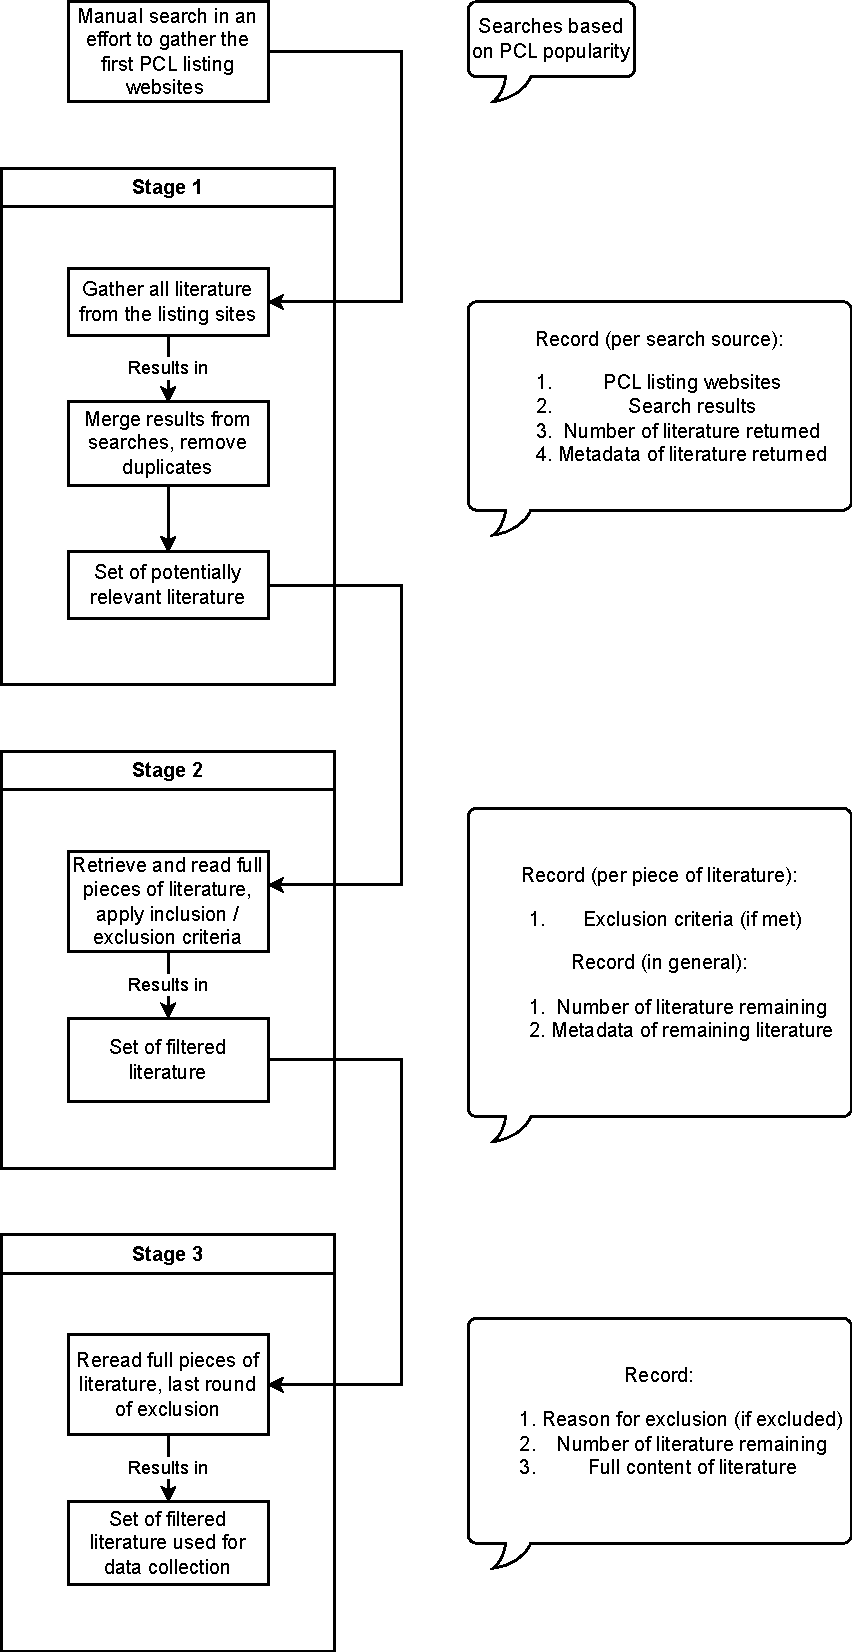
\includegraphics[scale=0.67]{figures/search-process.pdf}
	\caption{Search process divided into stages}
	\label{fig:search-process}
\end{figure}

% first stage
In the first stage, the search was conducted using the web pages titled  ''MIT License'' \citep{wikipedia:mit}, ''SPDX License List'' \citep{spdx:licenses}, ''The DFSG and Software Licenses'' \citep{debian:dfsg}, FSF's ''Category:License'' Wiki page \citep{fsf:licenselist}, GNU's ''Various Licenses and Comments about Them'' \citep{gnu:licenselist} and "OSI Approved licenses" \citep{osi:licenselist} focusing, focusing on the license listing site name and shortcode. Then we identified and eliminated any duplicates, producing a preliminary set of potentially relevant literature. The dataset after the first stage of the search process is provided in this thesis' repository \citep{mscthesis} under the name of \texttt{stage1-licenses.md}, as mentioned earlier.

%second stage
In the second stage, the inclusion and exclusion criteria were applied to further filter the literature and reduce the number of licenses to be reviewed. Then the resulting dataset was taken for a closer look where the quality of the literature was examined manually by the author, resulting in some manual exclusions based on the content and availability of the literature. This is where the inclusion and exclusion string took concrete place in which means the results were cross-referenced with the quasi-gold standard to validate it. The verbal reasoning for manual exclusions is clarified in \hyperref[incexc-criteria]{Sub-chapter 2.4}. The dataset after the second stage is provided in this thesis' repository \citep{mscthesis} under the name of \texttt{stage2-licenses.md}.

% third stage
The third stage was the most time-consuming and involved a manual review of the full license texts. After reading and evaluating each license, a final round of exclusions was completed and documented. The remaining licenses were used for data collection and analysis in the final part of the study. The final list of licenses is available in \hyperref[appendix:a]{Appendix A}.

% fetch licenses from scancode
\section{Inclusion and exclusion criteria\label{incexc-criteria}}
Before we could apply the inclusion and exclusion criteria to the literature we had to fetch the full license texts from somewhere since the first stage's dataset included only the shortcode and listing site name. We decided that the public license database by ScanCode published in GitHub \citep{scancode} was to be used fetching the initial full license texts based on the shortcodes of the first stage. The license database could be found by searching GitHub with the term ''license database''. The monolithic Python script used for this matching and fetching is provided in this thesis' repository \citep{mscthesis} under the name of \texttt{methods.py}. Some shortcodes from the first stage did not match any full license texts from the license database. We had to manually fetch the missing full license texts from these license listing sites. The fetching was done systematically in cycles until no more missing full license texts were found with the help of the first stage spreadsheet. as can be seen from the Python script. We now had a complete Python dictionary with the shortcode as the key and full license text as the value.

% incl excl regex string
To be eligible for the data collection and analysis, a license had to match the following inclusion and exclusion regular expression string:
\begin{verbatim}
  ^(?!.*\b(documentation\s+license|creative\s+commons|open data)\b).*
\end{verbatim}

% comments on applying
The regular expression string first included some inclusion matching but we soon realized it would be more efficient to exclude licenses than to include licenses. To establish the quasi-gold standard we first tried to exclude all full license texts including the words ''creative commons'' since we knew the Creative Commons licenses are not suitable for computer code, which is our scope. We then opened all excluded licenses into tabs in our text editor which the Python script assigned to their respective directory of excluded licenses based on the regular expression. We then looked quickly at the first few lines of the full license texts and judged if the license was indeed not suitable for our scope. Then we did the same to the included licenses in their respective directory and glanced if there were some types of licenses that were not suitable for our scope. We did one more cycle like this to finally exclude the string ''documentation license'' as well. During the two cycles we manually marked some licenses as included or excluded regardless of the regular expression matching since there did exist some corner cases the matching missed. This ended the second stage of search process which focused on inclusion and exclusion criteria.

% what was done to answer rq (table data extraction form)
\section{Data collection and data analysis}
To answer the research questions of this thesis, a thorough examination of the selected primary literature was conducted and the necessary data was collected using data extraction form presented in \hyperref[table:extraction]{Table 2.2}. A record of the full license texts after the third stage was kept for anaysis and is available as a directory called \texttt{stage3-licenses} in the thesis' repository \citep{mscthesis}.

\begin{table}[t]
	\begin{center}
		\begin{tabular}{||c c c||} 
			\hline
			\# & Field & Concern/Research question \\
			\hline
			F1 & Shortcode & RQ2, RQ3 \\
			F2 & Listing site name & RQ1, RQ2 \\
			F3 & Full text &  Documentation\\
			\hline
		\end{tabular}
		\caption{Data extraction form}
		\label{table:extraction}
	\end{center}
\end{table}

% third stage how to
To get the necessary from the remaining literature we decided that the next reasonable step was to remove duplicates from the licenses as systematically as possible. We used Python's \texttt{difflib} library to sort the full license texts. The library itself used the Ratcliff and Obershelp algorithm compare every full license text to every full license text. The time complexity is $O(n^3)$ and $\theta(n^2)$. This took our working computer 68 minutes each time the algorithm ran so we decided to only do one cycle of this type of duplicate removal. The licenses were outputted to \texttt{duplicate-finding} directory with the naming convention of \texttt{n-shortcode.txt} where the n was the sort order given by the Ratcliff and Obershelp algorithm. We then opened these licenses to tabs in our text editor and compared the full license texts by human eyes if they were actually the same license with little to no noise difference in the full license texts. The comparison tool of our text editor was also a helpful automation tool for longer licenses that could not fit into one computer display as whole without scrolling. ''open data'' was also applied in the regular expression string at this stage. While this should have happened in stage 2, we wanted to be honest that this exclusion really did happen in stage 3. At this stage we also manually excluded individual licenses from the final dataset if there was too much noise. For example, GNU listed licenses often as whitespaces or something alike.  Examples of these will be given in \hyperref[results]{Chapter 3}. This ended the third stage of the search process and provided us with the necessary data to answer the research questions.

%  next chapter presents outcomes
The subsequent chapter presents the outcomes of the steps taken in the study, as discussed above.